\documentclass[a4paper]{article} 
\addtolength{\hoffset}{-2.25cm}
\addtolength{\textwidth}{4.5cm}
\addtolength{\voffset}{-3.25cm}
\addtolength{\textheight}{5cm}
\setlength{\parskip}{3pt}
\setlength{\parindent}{0in}

%----------------------------------------------------------------------------------------
%	PACKAGES AND OTHER DOCUMENT CONFIGURATIONS
%----------------------------------------------------------------------------------------

\usepackage{charter} % Use the Charter font
\usepackage[utf8]{inputenc} % Use UTF-8 encoding
\usepackage{microtype} % Slightly tweak font spacing for aesthetics
\usepackage[english, ngerman]{babel} % Language hyphenation and typographical rules
\usepackage{amsthm, amsmath, amssymb} % Mathematical typesetting
\usepackage{float} % Improved interface for floating objects
\usepackage{hyperref, xurl} % For hyperlinks in the PDF
\usepackage{graphicx, multicol} % Enhanced support for graphics
\usepackage{xcolor} % Driver-independent color extensions
\usepackage{marvosym, wasysym} % More symbols
\usepackage{rotating} % Rotation tools
\usepackage{censor} % Facilities for controlling restricted text
\usepackage{listings, style/lstlisting} % Environment for non-formatted code, !uses style file!
%\usepackage{pseudocode} % Environment for specifying algorithms in a natural way
\usepackage{algorithm}
\usepackage{algorithmic}
\usepackage{array}
\usepackage{multirow}
\usepackage{makecell}
\usepackage{pdfpages}
%\usepackage{style/avm} % Environment for f-structures, !uses style file!
\usepackage{booktabs} % Enhances quality of tables
\usepackage{tikz-qtree} % Easy tree drawing tool
\tikzset{every tree node/.style={align=center,anchor=north},
         level distance=2cm} % Configuration for q-trees
%\usepackage{style/btree} % Configuration for b-trees and b+-trees, !uses style file!
\usepackage[backend=biber,style=numeric,
            sorting=nyt]{biblatex} % Complete reimplementation of bibliographic facilities
\addbibresource{ecl.bib}
\usepackage{csquotes} % Context sensitive quotation facilities
%\usepackage[yyyymmdd]{datetime} % Uses YEAR-MONTH-DAY format for dates
%\renewcommand{\dateseparator}{-} % Sets dateseparator to '-'
\usepackage{fancyhdr} % Headers and footers
\pagestyle{fancy} % All pages have headers and footers
\fancyhead{}\renewcommand{\headrulewidth}{0pt} % Blank out the default header
\fancyfoot[L]{} % Custom footer text
\fancyfoot[C]{} % Custom footer text
\fancyfoot[R]{\thepage} % Custom footer text
\newcommand{\note}[1]{\marginpar{\scriptsize \textcolor{red}{#1}}} % Enables comments in red on margin

\newcommand{\classname}[1]{\texttt{#1}}
\newcommand{\highlight}[1]{\textbf{#1}}

\long\def\citacao#1{\medskip % \citacao is the command
	\begingroup
	\parindent 0pt
	\leftskip=1.27cm
	\small #1 \par \medskip
	\endgroup
}
%----------------------------------------------------------------------------------------

\begin{document}

%-------------------------------
%	TITLE SECTION
%-------------------------------

\fancyhead[C]{}
\hrule \medskip % Upper rule
\begin{minipage}{0.295\textwidth} 
\raggedright
\footnotesize
Robert Roth \hfill\\   
Sommersemester 2025\hfill\\  
\end{minipage}
\begin{minipage}{0.4\textwidth} 
\centering 
\large 
Übung 02\\ 
\normalsize 
Spieleprogrammierung\\ 
\end{minipage}
\begin{minipage}{0.295\textwidth} 
\raggedleft
\today\hfill\\
\end{minipage}
\medskip\hrule 
\bigskip



\section{Einleitung}
In dem zweiten Teil dieser Portfolioprüfung sollte ein nicht-spielbarer Charakter (NPC, engl. \textit{non-playable character}) erstellt werden, der eine gewisse Menschenähnlichkeit hat. Dieser Charakter soll verschiedene Animationen und Bewegungsarten beherrschen. Jedoch soll das Verhalten nicht komplett geskriptet sein, sondern von einer generativen KI gesteuert werden. 

In meiner Lösung habe ich die API-Schnittstelle von OpenAI verwendet, um das gewünschte Verhalten umzusetzen.  Dafür werden Daten über den NPC und den Spieler per REST-API an die KI gesendet und die Antwort entsprechend geparset und umgesetzt. 

Der Bericht beschreibt die entwickelte Lösung, beginnend mit der Erfassung des NPC-Zustands, über die Kommunikation mit dem KI-Modell, bis hin zur Umsetzung der vorgeschlagenen Reaktion in der Spielwelt. Darüber hinaus werden die dabei auftretenden Herausforderungen und deren Lösungsansätze erläutert.

\section{Der NPC}
Auf der Suche nach einem passenden NPC im Unity Asset Store bin ich auf ein Package von Mocap Central gestoßen, was meinen Anforderungen schon sehr nahe kam.\footnote{Siehe \url{https://assetstore.unity.com/packages/3d/animations/mc-sample-believable-3d-animations-by-mocap-central-291284}} Das Package besitzt bereits ein Prefab für einen menschenähnlichen Charakter und bietet viele Animationen zum Testen an (siehe \autoref{fig:npc}).
\begin{figure}[h]
	\centering
	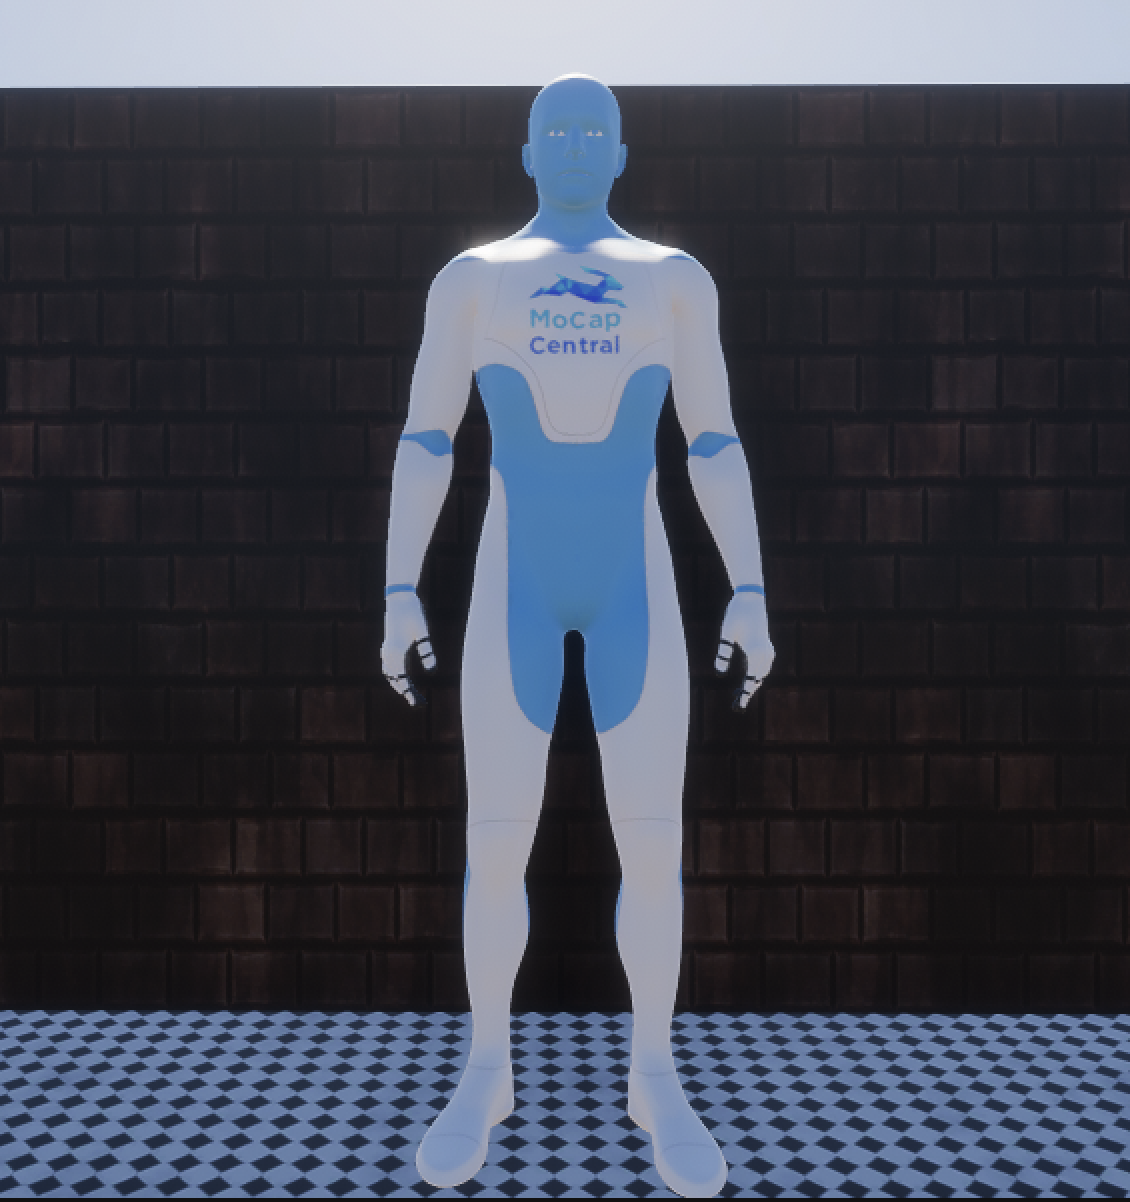
\includegraphics[width=.5\textwidth]{img/NPC.png}
	\caption{Der NPC-Charakter des verwendeten Packages.}
	\label{fig:npc}
\end{figure}


\subsection{Die Animationen}
Für die Darstellung realistischer Verhaltensweisen stand eine Vielzahl einzelner Animationsclips zur Verfügung, die spezifische Bewegungen wie Gehen oder Emotionen wie Weinen abbildeten. Viele dieser Clips enthielten auch vorbereitende „Unter-Animationen“, etwa das Hinknien vor dem Kriechen oder das Aufrichten danach. Allerdings reichten diese Einzelanimationen allein nicht aus, um ein konsistentes und nachvollziehbares Verhalten des NPCs zu erzielen. In diesem Projekt sind die Animationen Idle, Gehen, Rennen, Kriechen und Weinen möglich.

\begin{figure}[h]
	\centering
	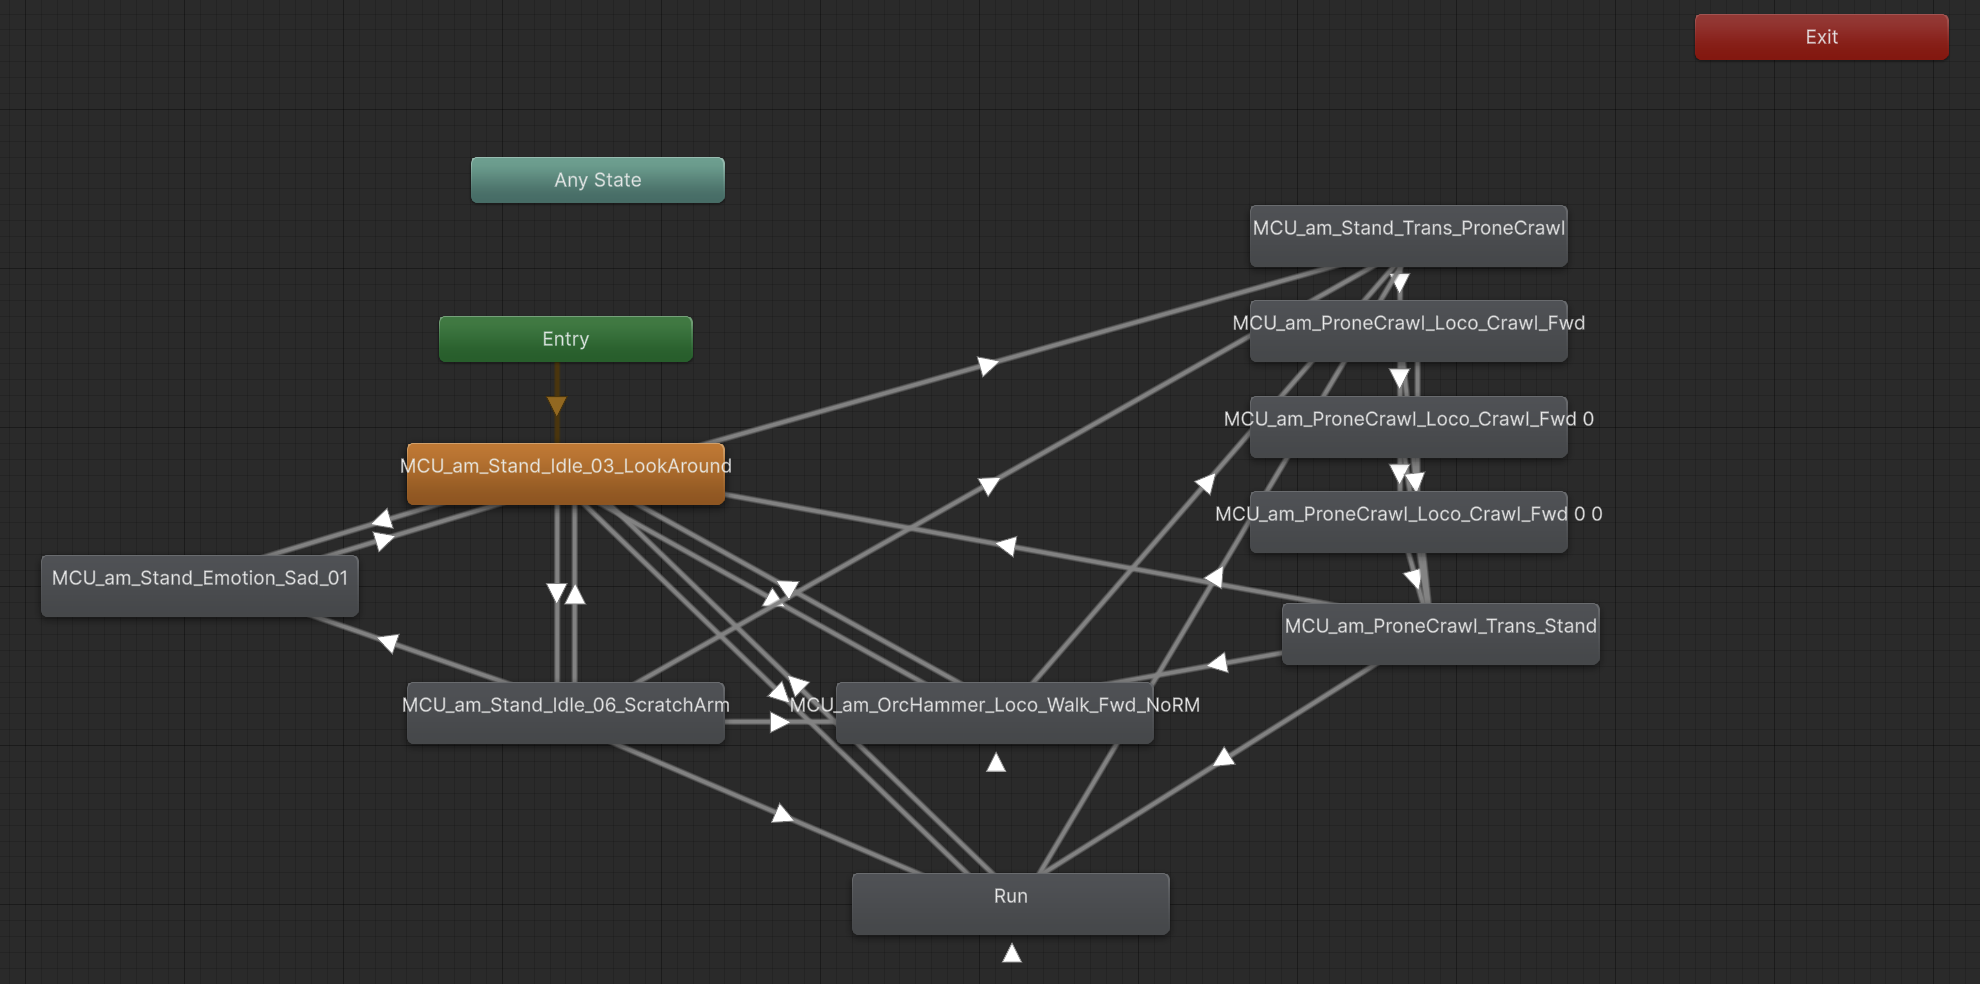
\includegraphics[width=.7\textwidth]{img/Animatorcontroller.png}
	\caption{Animator-Controller des NPC, der die Übergänge zwischen den einzelnen Animationen anzeigt. Von links nach rechts befinden sich die Animationen für: Weinen, Idle, Gehen und Rennen, Kriechen.}
	\label{fig:animatorcontroller}
\end{figure}

Deshalb mussten alle Animationsclips in einem zentralen Animator-Controller zusammengefasst werden (siehe \autoref{fig:animatorcontroller}). Nur so war es möglich, saubere Übergänge zwischen den Animationen zu definieren, die sich dynamisch an den aktuellen Zustand und die empfangenen Aktionen der KI anpassen. Im Animator wurden die Zustände mit Triggern und Parametern verbunden, um nahtlose Übergänge wie das Wechseln vom Idle in die Kriech- oder Laufbewegung zu ermöglichen. Besonders wichtig war dabei die Steuerung von Spezialanimationen, die nur unter bestimmten Bedingungen abgespielt werden dürfen, beispielsweise das Hinknien vor dem Kriechen oder das Aufstehen danach.

Erst durch diese gezielte Kombination von Einzelanimationen mit einem fein abgestimmten Animationsgraphen entstand ein glaubhaftes Bewegungsverhalten, das dem KI-gesteuerten NPC ermöglicht, je nach Spielsituation fließend und glaubwürdig zwischen den Verhaltensweisen zu wechseln.

Allerdings gab es auch Hindernisse. In dem verwendeten Package sind keine Animationen für reguläres Gehen oder Laufen, stattdessen gibt es nur eine Gehanimation für einen Orc. Da es keine Vorgaben gab, wie der NPC gehen soll, ist das seine Gehanimation in diesem Projekt. Um das Laufen darzustellen, wurde dann diese Gehanimation auf 2,5-facher Geschwindigkeit abgespielt. So kann zumindest erahnt werden, dass es eine Laufanimation darstellen soll. 

\subsection{Die Translation}
Die Animationen sind ein entscheidener Faktor, um eine Bewegung darzustellen, aber der Charakter muss auch die Position verändern, um sich tatsächlich zu bewegen. Glücklicherweise war die Translation bereits in der Kriech-Animation integriert, wodurch hier etwas weniger Arbeit angefallen ist. Allerdings bestehen die Geh- und Laufbewegung nur aus der Animation selbst, weswegen hier die Translation mit Unity-Skripten implementiert wurde.

Um die Bewegung auch nutzbar zu machen wurden die Methoden \texttt{WalkTo(Vector3)}, \texttt{RunTo(Vector3)} und \texttt{CrawlTo(Vector3)} implementiert. Da die Methoden nahezu ähnlich verlaufen, werde ich als Beispiel WalkTo erklären. Wenn die Methode WalkTo aufgerufen wird, dann beginnt der NPC damit sich zunächst in die Richtung zu drehen, in der er sich bewegen will. Sobald die Rotation beendet ist, beginnt die Gehanimation sowie die Translation zur gewünschten Koordinate. Dabei kann die y-Koordinate allerdings nicht beeinflusst werden, da der NPC nicht schweben können soll und es glücklicherweise auch keine Treppen oder ähnliches im Labyrinth gibt. Wenn die gewünschte Position erreicht ist, wechselt der NPC automatisch wieder in die Idle-Animation zurück. Die Laufbewegung ist ähnlich zur Gebewegung, allerdings wird die Animation auf 2,5-facher Geschwindigkeit abgespielt.

\section{Die KI}
In der Aufgabenstellung war gefordert, dass der NPC sich nicht geskriptet verhalten soll, sondern stattdessen von einer KI gesteuert werden soll. Ich habe mich hierbei für die KI-Schnittstelle von OpenAI entschieden. Ich möchte zunächst darauf eingehen, wie die aktuelle Kommunikation mit der KI aufgebaut ist und dann im Nachgang diese Entscheidung erklären und auf verschiedene Hindernisse eingehen.

\subsection{Der Aufbau}
Zu Beginn des Programms wird einmal eine längere Erklärung und das aktuelle Labyrinth an die KI gesendet. Die KI soll dann zunächst nur mit dem Befehl zu einer Idle-Animation reagieren, um zu bestätigen, dass sie die Aufgabe verstanden hat. Gewünscht ist, dass die KI nur im JSON-Format antwortet, sodass die Nachricht leicht verarbeitet und umgesetzt werden kann. Der initiale Prompt sieht so aus:

\citacao{Du bist ein NPC in einem 3D-Labyrinth. Das Labyrinth ist aus einer ASCII-Textdatei generiert, in der gilt:\\
	Die txt-Datei wird dir immer vollständig mitgeschickt. Jede Zeile stellt eine Z-Reihe dar.  \\
	Die oberste Zeile in der ASCII-Datei entspricht Z=0, jede weitere Zeile erhöht Z um 1 (Z=1, Z=2 usw.).  \\
	Die Zeichen in jeder Zeile repräsentieren die X-Positionen: Der linke Buchstabe ist X=0, der rechte Buchstabe ist X=mazeWidth-1. \\
	Die Y-Position ist immer konstant auf 1, da das Labyrinth nur auf einer Ebene liegt. Alle Koordinaten haben daher die Form X,1,Z.\\
	Die Bedeutungen der ASCII-Zeichen sind:
	
	- \# steht für eine Wand, die nicht durchquert werden darf.\\
	- M steht für eine metallische Wand (ebenfalls blockiert).\\
	- G steht für Glas (blockiert, auch wenn durchsichtig).\\
	- . ist begehbarer Boden.\\
	- P ist die Position des Spielers.\\
	- N ist die Startposition des NPC.
	
	Die Koordinaten aller Zeichen mit \#, M oder G gelten als blockiert. Eine geplante Bewegung darf keine dieser Koordinaten durchqueren oder darauf enden.\\
	Die Bewegung erfolgt immer in einer geraden Linie vom Startpunkt zum Ziel -- kein Teleportieren und kein Durchqueren blockierter Felder.\\
	Bevor du eine Bewegung planst, überprüfe, dass alle Zwischenpositionen zwischen Start- und Zielpunkt frei von blockierten Feldern sind.  \\
	Du darfst frei handeln.\\
	Mögliche Aktionen, die du ausgeben darfst, sind:
	
	- \{``action'': ``walk'', ``target'': \{``x'': X, ``y'': 1, ``z'': Z\}\}\\
	- \{``action'': ``run'', ``target'': \{``x'': X, ``y'': 1, ``z'': Z\}\}\\
	- \{``action'': ``crawl'', ``target'': \{``x'': X, ``y'': 1, ``z'': Z\}\}\\
	- \{``action'': ``cry''\}\\
	- \{``action'': ``idle''\}
	
	Dabei gilt:\\
	- Die Aktionen walk, run und crawl MÜSSEN IMMER ein target haben. Du kannst diese Aktionen nicht ausführen, ohne eine target Position anzugeben!\\
	- Du darfst keine Aktion ausgeben, die dich durch Wände (\#) führt.\\
	- Gehe davon aus, dass (0,0,0) immer außerhalb des Spielfelds ist.\\
	- Gib Bewegungen immer als JSON mit drei separaten Schlüsseln an: \{``x'': X, ``y'': 1, ``z'': Z\}.\\
	- Verwende als target NICHT position als String wie ``target'': \{``position'': ``(X, Y, Z)''\}.\\
	- Wenn du dich bewegen möchtest, gib die Zielposition als ganzzahlige Koordinaten an.\\
	- Wenn du weinen oder idle bleiben willst, gib keine Zielposition an.\\
	- Ich sende dir regelmäßig die Position und Rotation deines Charakters, sowie die Position des Spielercharakters.\\
	- Gib die Antwort AUSSCHLIESSLICH als JSON-Objekt zurück, ohne zusätzliche Erklärungen oder Kommentare.
	- Antworte nicht im Fließtext.\\
	- Antworte immer genau in diesem JSON-Format, ohne jegliche Abweichung oder Zusätze.\\
	- Beginne, indem du mit einer Idle-Action antwortest!\\
	Hier ist das aktuelle Labyrinth:
}

Nachdem der initiale Prompt gesendet wurde, wird im 10-Sekunden-Takt die aktuelle Position des Spielers, sowie die Position und Rotation des NPCs an die KI gesendet. Der Prompt dafür sieht wie folgt aus:

\citacao{Aktueller Zustand: \\
	NPC Position: (X, Y, Z) \\ 
	NPC Rotation: (X, Y, Z)  \\
	Spieler Position: (X, Y, Z)\\
	Gib nur ein JSON mit einer der folgenden Aktionen zurück: walk, run, crawl, cry, idle.\\
	Die Aktionen walk, run und crawl MÜSSEN IMMER ein target haben.\\
	Gib das target immer als JSON mit drei separaten Schlüsseln an: \{``x'': X, ``y'': 1, ``z'': Z\}.\\
	Benutze jede Aktion gleich oft! Du darfst die gleiche Aktion nicht zwei Mal in Folge wählen.
}

Wenn die KI dann auf diese Prompts anwortet, dann wird diese Antwort entsprechend verarbeitet. Dafür wird die Antwort zunächst aus dem JSON-Format heraus in ein Objekt der Klasse \texttt{ResponseData} gewandelt. Dieses Objekt speichert als Variablen einen String \texttt{action} und die entsprechende Position, wo sich ggf. hinbewegt werden soll. Der Ablauf ist in \autoref{fig:uml} dargestellt.

\begin{figure}[h]
	\centering
	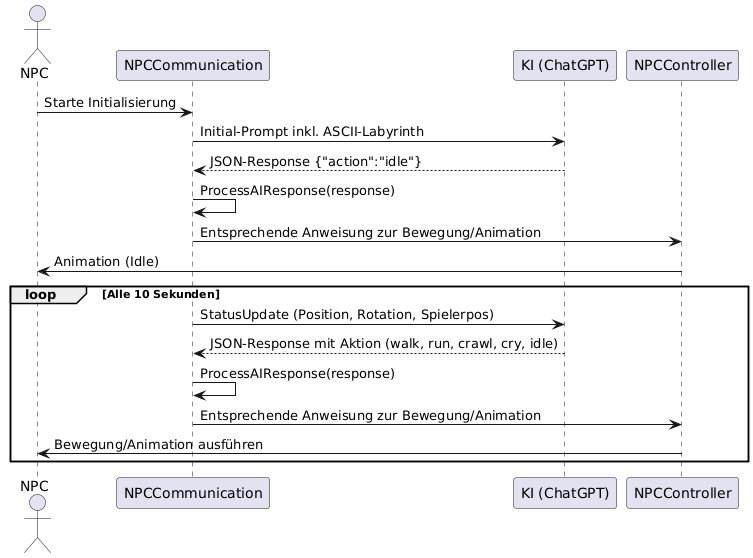
\includegraphics[width=.7\textwidth]{img/UML.png}
	\caption{UML-Sequenzdiagramm, was die Kommunikation mit der KI darstellt.}
	\label{fig:uml}
\end{figure}

\subsection{Schwierigkeiten}
Im folgenden Abschnitt würde ich gerne auf die Probleme und Schwierigkeiten eingehen, die mir die KI bereitet hat. Zuerst gehe ich dabei auf die Wahl der KI ein. 

Da von der Arbeitsgruppe eine DeepSeek-Instanz zur Verfügung gestellt wurde, die für die Abgabe benutzt werden kann, war es zunächst natürlich naheliegend diese KI zu verwenden. Allerdings habe ich keinen Prompt gefunden, mit der die KI so reagiert hat, dass ich es verwenden könnte. Egal wie sehr ich der KI gesagt habe, dass sie bitte ausschließlich als JSON antworten soll, es kam immer ein viel zu langer Fließtext zurück. Diese Fließtext zu parsen und analysieren hätte mehr Aufwand gekostet, als den NPC selbst zu programmieren, weswegen das keine Option war.\\
Mein nächster Gedanke war, dass ich die API von OpenAI verwenden könnte, da ich auch ChatGPT im Alltag am ehesten verwende. Außerdem ist es möglich bereits mit 5\$ Guthaben bei der OpenAI-API relativ viele Anfragen zu stellen, weswegen ich es gerne ausprobieren wollte. Allerdings stand ich jetzt vor der Wahl, an welches Model ich die Anfragen senden möchte. Ich habe die Modelle GPT4o Mini, GPT4.1 Nano, GPT4.1 Mini, O4 Mini und chatgpt 4o-latest ausprobiert. Die Ergebnisse waren alle relativ ähnlich, weswegen ich mich für GPT4o Mini entschieden habe, weil dort die Anfragen im Vergleich mit den anderen getesteten Modellen am günstigsten sind. 

Dennoch ist auch diese KI keine optimale Lösung. Es kommt zu drei Problemen:
\begin{enumerate}
	\item Die KI tendiert dazu, nur walk zu verwenden.
	\item Sie ignoriert Wände und andere Hindernisse.
	\item Die KI gibt die Zielposition gerne im falschen Format an.
\end{enumerate}
Beide Probleme wurden im Prompt eigentlich angesprochen. Obwohl in jedem Status-Prompt steht \glqq Benutze jede Aktion gleich oft! Du darfst die gleiche Aktion nicht zwei Mal in Folge wählen.\grqq\ wählt die KI jedes Mal walk. Auch steht im initialen Prompt geschrieben, wie das Labyrinth aufgebaut ist und wo die Wände sind und dass die Wände nicht überschritten werden dürfen. Trotzdem ignoriert sie diese Wände in der Regel. Wenigstens die äußersten Wände des Labyrinths hat die KI in meinen Tests bisher nicht verlassen. Auch gibt sie gerne das Format der Zielposition falsch an, obwohl klar definiert ist, wie sie reagieren soll. Gefordert ist, dass sie die X-, Y- und Z-Position einzeln zurückgibt. Im Test ist es allerdings häufiger vorgekommen, dass sie stattdessen einen Vektor \texttt{position} zurückgegeben hat.

Da stellt sich mir die Frage: Ist die KI nicht in der Lage es besser zu machen, oder benötige ich einen besseren Prompt? Leider habe ich keine Antwort auf die Frage, aber ich möchte glauben, dass das Problem bei der KI liegt.

\section{Fazit}
Mit der Anbindung des NPCs an ein KI-Modell konnte ein NPC-Verhalten umgesetzt werden, das sich dynamisch an den Spielzustand anpasst und nicht ausschließlich durch vordefinierte Skripte gesteuert ist. Die gewählte Lösung ermöglichte es, den aktuellen Zustand des NPCs und der Spielwelt regelmäßig an die KI zu übermitteln und so auf Basis der KI-Antwort geeignete Aktionen wie Gehen, Rennen, Kriechen oder emotionale Reaktionen wie Weinen auszulösen.

Die wesentliche Herausforderung bestand darin, die KI durch einen präzisen Prompt so zu steuern, dass sie konsistente JSON-Antworten liefert, die sich direkt in Unity verarbeiten lassen. Außerdem mussten die Übergänge zwischen den Animationen im Animator-Controller so gestaltet werden, dass sie fließend und glaubwürdig wirken. Ein robustes Fehlerhandling stellte sicher, dass auch unvollständige oder fehlerhafte KI-Antworten das Spiel nicht zum Absturz bringen.

Die Umsetzung hat gezeigt, dass ein KI-gesteuerter NPC zwar ein netter Ansatz ist, aber doch wesentlich mehr Arbeit benötigt, als einen simplen Prompt. Es braucht viel Feinarbeit bei der Erstellung des Prompts und selbst dann ist die Antwort der KI nicht immer vorhersehbar. Trotzdem war es ein spannendes Experiment um zu sehen, wie weit man mit einer simplen Anfrage kommt.

\end{document}
